%!TEX root = syntheyes15.tex

\section{Rendering photo-realistic training images}

% define each rendered image by c, g, L
Once our eye-region model is prepared, we render it from a wide range of camera positions and lighting conditions.
%
We briefly describe how we use image-based lighting \cite{debevec2002image} to model a wide range of realistic lighting conditions, and finally discuss the details of our rendering setup.

We position the camera using spherical coordinates about the eyeball centre. 

At each camera position, we iterate over a range of eye gaze vectors to synthesize eye images 

All images are rendered with an orthgraphic camera model, as this simulates an eye-region image being cropped from an already wide-angle camera image, e.g. webcam.

\begin{figure}
    \centering
    \begin{subfigure}[t]{0.48\columnwidth}
        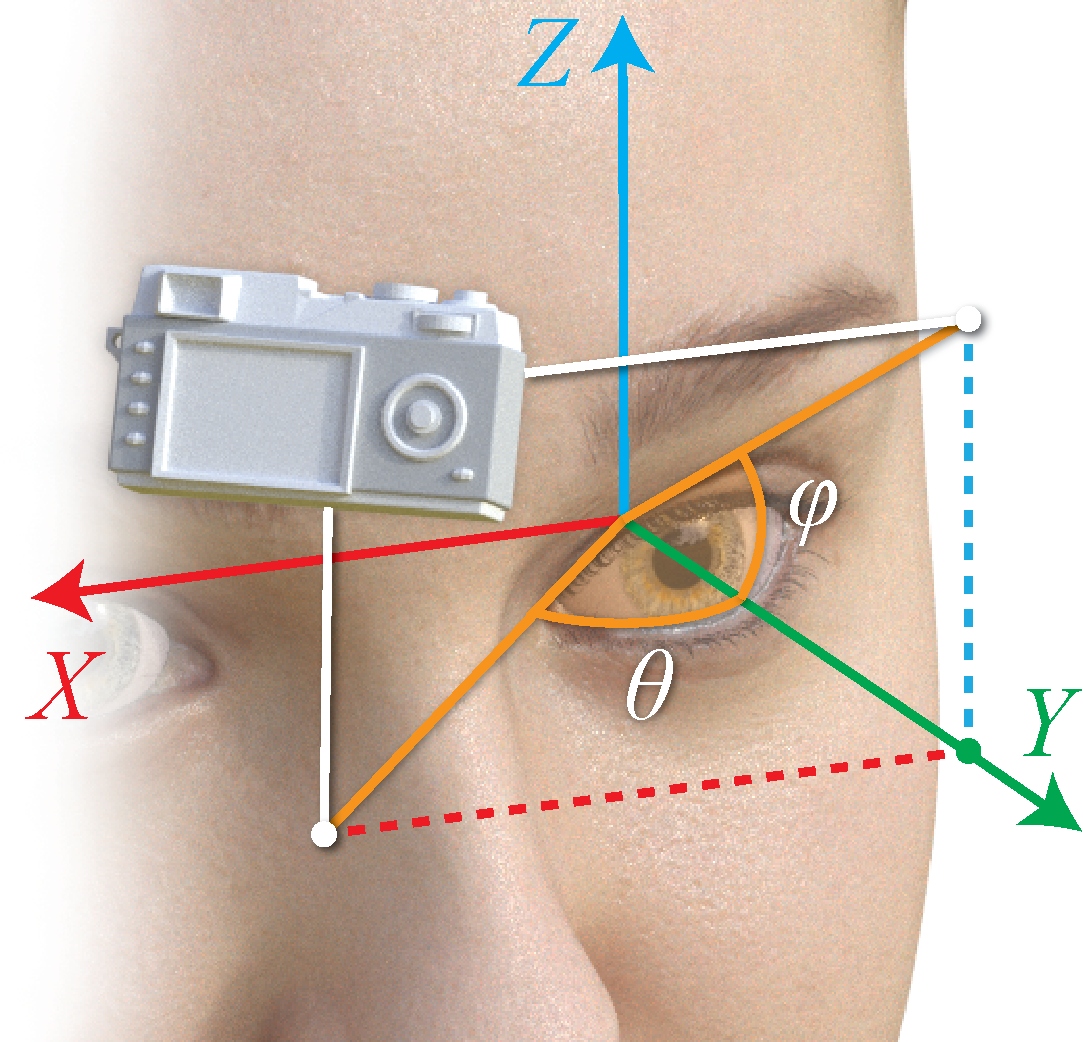
\includegraphics[width=\textwidth]{camera_position}
        \caption{The camera is positioned using spherical coordinates}
        \label{fig:cam_pos_spher_coords}
    \end{subfigure}
    \hfill
    \begin{subfigure}[t]{0.48\columnwidth}
        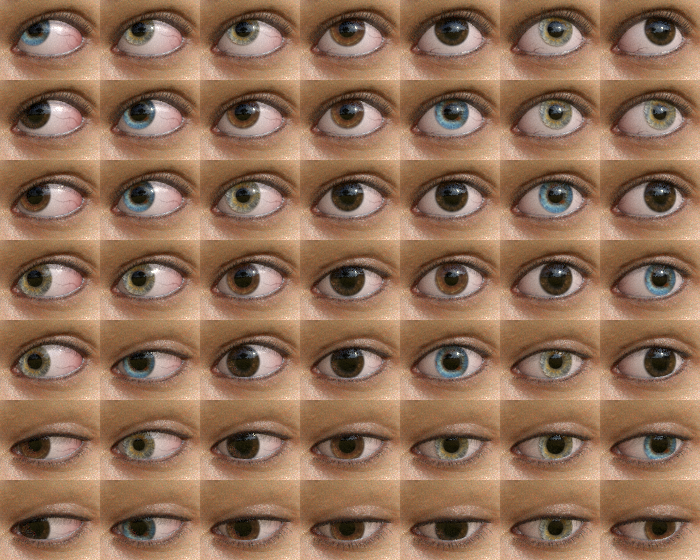
\includegraphics[width=\textwidth]{camera_pos_sample_renders_7x7}
        \caption{Example renderings from one camera position}
        \label{fig:cam_pos_example_renders}
    \end{subfigure}
    \caption{\ref{fig:cam_pos_spher_coords} shows how we position the camera to simulate changes in head pose. At each camera position, we render many eye images (\ref{fig:cam_pos_example_renders}) by posing the eyeball model.}
    \label{fig:cam_pos}
\end{figure}

\subsection{Lighting}

One of the hardest problems for computer vision systems is 

We 

\begin{figure}
    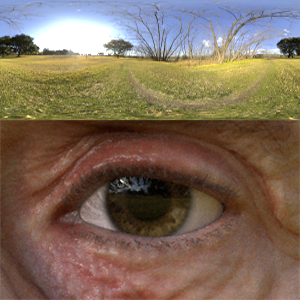
\includegraphics[width=0.24\columnwidth]{fig_env_1} \hfill
    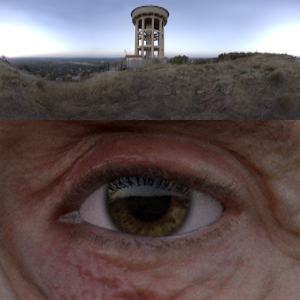
\includegraphics[width=0.24\columnwidth]{fig_env_2} \hfill
    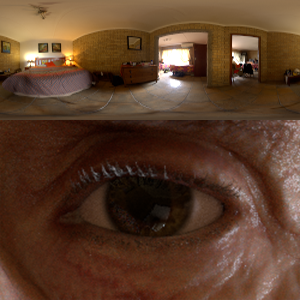
\includegraphics[width=0.24\columnwidth]{fig_env_3} \hfill
    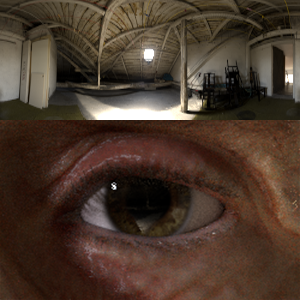
\includegraphics[width=0.24\columnwidth]{fig_env_4}
    \caption{Appearance variation from lighting is modelled with poseable high-dynamic-range environment maps \cite{debevec2002image}.}
    \label{fig:participants}
\end{figure}

\subsection{Computational setup}

We can rapidly generate diverse datasets much faster than manual collection and annotation.